\subsection{Funkcje Skalarne i Tabelarne}

Zostały stworzone następujące funkcje:
\begin{itemize}
	\item \href{run:Sources/SQL/3. Funkcje Skalarne/017_Utworzenie_funkcji_wyliczajacej_koszt_najmu.sql}{\texttt{koszt\_najmu} - Funkcja obliczająca koszt danego najmu}
\end{itemize}

\subsubsection{\texttt{koszt\_najmu} - Funkcja obliczająca koszt danego najmu}

|koszt_najmu (@najem_id int)| - Funkcja ta oblicza koszt konkretnego najmu wskazanego w parametrze |@najem_id|, zwracana wartość ma typ |DECIMAL(15, 2)| który jest kompatybilny z typem kolumny \texttt{koszt} w tabeli \texttt{}najmy. Przykład wykorzystania tej funkcji jest w triggerze z listingu \ref{lst:trigger-wylicz_koszt_najmu}.

%\begin{figure}[h]
%	\centering
%    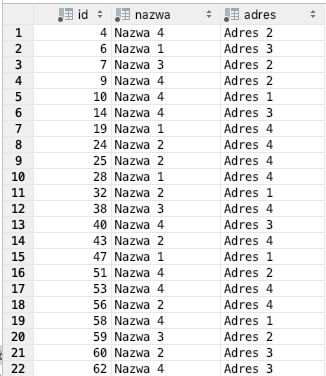
\includegraphics[width=0.4\textwidth]{lista_niepopularnych_obiektow}
%	\caption{Wyświetlony widok \texttt{lista\_niepopularnych\_obiektow}}
%	\label{fig:lista_niepopularnych_obiektow}
%\end{figure}

\begin{lstlisting}[language=SQL, caption={Skrypt tworzący funkcję skalarną \texttt{koszt\_najmu}}, label={lst:function-koszt_najmu}]
CREATE FUNCTION koszt_najmu (@najem_id INT)
  RETURNS DECIMAL(15, 2)
  AS
  BEGIN
		DECLARE @dzienna_stawka DECIMAL(10,2);
		DECLARE @data_rozpoczecia DATE;
		DECLARE @data_zakonczenia DATE;

    SELECT @dzienna_stawka = o.dzienna_stawka_najmu,
           @data_rozpoczecia = n.data_rozpoczecia,
           @data_zakonczenia = data_zakonczenia
      FROM najmy n
      JOIN obiekty o on n.obiekt_id = o.id
      WHERE n.id = @najem_id;

    IF @data_zakonczenia IS NULL
      RETURN NULL;

    RETURN (1+DATEDIFF(DAY, @data_rozpoczecia, @data_zakonczenia))*@dzienna_stawka;
  END
\end{lstlisting}